%%%%%%%%%%%%%%%%%%%%%%%%%%%%%%%%%%%%%%%%%%%%%%%%%%%%%%%%%%%%%%%%%%%%%%%%%%%%%%%%%%%%%%%%%%%%%%%%%%%%%%%%%%%%
%%%%%%%%%%%%%%%%%%%%%%%%%%%%%%%%%%%%%%%%%%%%%%%%%%%%%%%%%%%%%%%%%%%%%%%%%%%%%%%%%
% \subsection{Control System}
% When the quadrotor is calibrated, armed and have multiple sensor readings, the control system initiates. A block diagram of the first control system used on the Plywood Quadcopter is provided in Fig. \ref{fig:dir}.
% \begin{figure}[H]
%           \centering
%             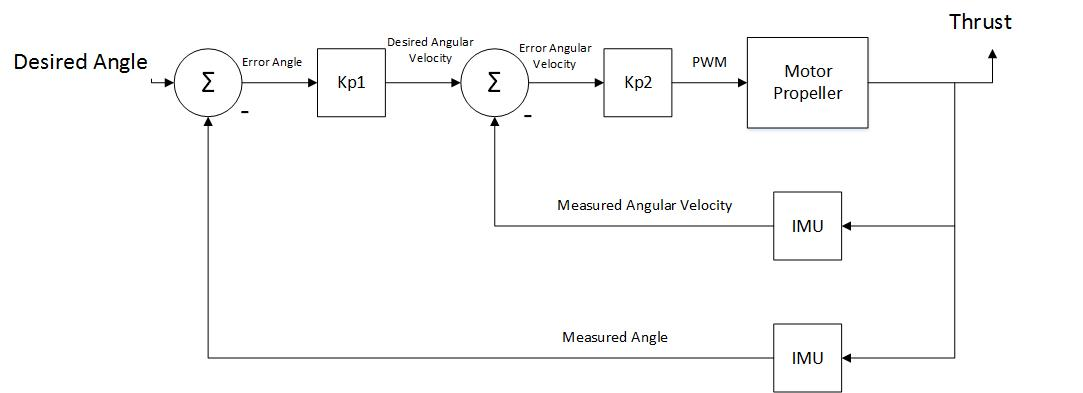
\includegraphics[scale = 0.62]{VAPIQ-PICTURES/CSBD.jpg}
%                 \caption{Proportional-Controller}
%                 \label{CSBD}
%             \label{fig:dir}
% \end{figure} 

% It first calculates the average of the sample data for angle and angular velocity. The angle error is calculated by taking the desired angle and subtracting the actual angle. 

% \begin{equation}
%   Angle Error = Desired Angle - Measured Angle
% \end{equation}

% By taking the error of the angle and multiplying it with a constant, the result will be the desired change in angular velocity. This is given that the constant is tuned properly.

% \begin{equation}
%   Desired Angular Velocity = Angle Error * Kp
% \end{equation}

% The bigger the error, the larger the compensation must be. The closer the quadcopter is to its desired position, the slower it needs to move. Taking the desired angular velocity and subtracting it from the actual velocity gives the change in angular velocity needed.

% \begin{equation}
%   Angular Velocity Error = Desired Angular Velocity - Measured Velocity
% \end{equation}


% The differential of thrust is given by the error in angular velocity multiplied with a constant.
% This number can give us the differential of force the quadcopter needs to correct on each axes. \\

% \begin{equation}
%   dThrust =   Angular Velocity Error * Kp2
% \end{equation}


% \begin{figure}[H]
%           \centering
%             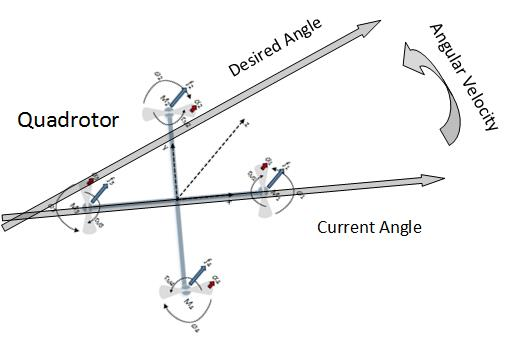
\includegraphics[scale = 0.67]{VAPIQ-PICTURES/OnBCS.jpg}
%                 \caption{Stability Control}
%                 \label{StabiilityControl}
%             \label{dir}
% \end{figure} 

% To give an specific example, if motor 1 and 3, 2 and 4 has a differential thrust of 20$\mu$s, and the thrust needed for hover is 1300$\mu$s: \bigskip
% $$motor1 = Hover (1300) + differential (20)$$ \\
% $$motor3 = Hover (1300) - differential (20)$$  \\
% \bigskip

% If the differential thrust is negative, motor 3 will increase and motor 1 will decrease. The PWM signals varies from 1000$\mu$s to 2000$\mu$s.


%%%%%%%%%%%%%%%%%%%%%%%%%%%%%%%%%%%%%%%%%%%%%%%%%%%%%%%%%%%%%%%%%%%%%%%%%%%%%%%
%
% Vanja Controller
%
%%%%%%%%%%%%%%%%%%%%%%%%%%%%%%%%%%%%%%%%%%%%%%%%%%%%%%%%%%%%%%%%%%%%%%%%%%%%%%%%





% \subsection{Autonomous Control System}
% The off-board control system computes the angles necessary to reach the desired position. This data is sent to the quadrotor. The autonomous system begins with storing the start position and the current time. \\

% The external computer constantly acquires the new position and rotation of the quadrotor. If no data is received a counter is increased, and the last position and rotation measured becomes the current. If this happens five times the quadrotor will stabilize and shutdown. If data is received the counter resets. \\
% When the off-board gets information from Qualisys it calculates the current velocity. The last position and time is updated as the current time and position. \\
% \\

% \begin{figure}[H]
%           \centering
%             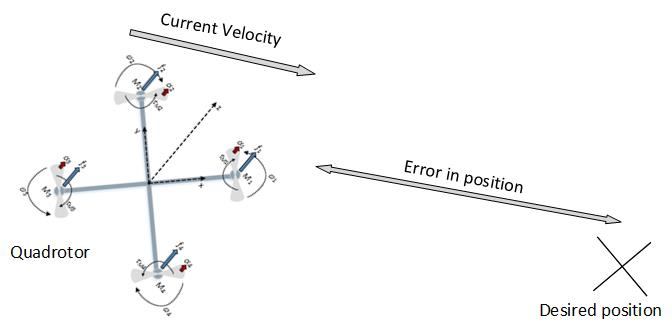
\includegraphics[scale = 0.67]{VAPIQ-PICTURES/OBCS.jpg}
%                 \caption{Trajectory Control}
%                 \label{TrajectoryControl}
%             \label{dir}
% \end{figure} 

% The next steps in this algorithm is very similar to how the fixed pitch quadrotor is stabilized. The first step is finding out the error in position. This is done by taking the desired position and subtracting the current. 

% \begin{equation}
%   Error Position = Desired Position - Measured Position
% \end{equation}

% Multiplying the desired position with a constant yields the value for the desired speed. 

% \begin{equation}
%   Desired Velocity = Error Position * Kp
% \end{equation}

% The desired speed will then change regarding to the distance. The further away from the desired position, the bigger roll and pitch angles are desired. The error between the desired speed is found by subtracting desired velocity from the measured velocity.

% \begin{equation}
%     Error Velocity = Desired Velocity - Measured Velocity
% \end{equation}

% This error in speed can be directly applied to the roll and pitch angles when multiplied with another constant. 

% \begin{equation}
%   dAngle =  Error Velocity * Kp2
% \end{equation}

% The thrust also gets computed in this algorithm. To get the thrust vectors in the X and Y directions, the thrust given is divided by $\cos$ to the respective angles. The combined thrust vector is found by adding components for X,Y and Z. The Z component can be found by taking the error in Z-position times a constant.  

% \begin{equation}
%         ThrustX = \frac{thrust}{cos(angularX)}
% \end{equation}

% \begin{equation}
%         ThrustY = \frac{thrust}{cos(angularY)}
% \end{equation}

% \begin{equation}
%         Thrust = \frac{thrustX + thrustY}{2}  + errorZ*kpZ
% \end{equation}

% The values computed needs to be limited in order to not exceed angles that cannot be flown in.
% All the data computed in the algorithm then gets sent to the quadrotor and the code rinse and repeats.


%%%%%%%%%%%%%%%%%%%%%%%%%%%%%%%%%%%%%%%%%%%%%%%%%%%%%%%%%%%%%%%%%%%%%%%%%%%%%%%%%%%%%%%%%%%%%%%%%%%%%%%%%%%%


%%   FLYTTET TIL  CONTROL SYSTEM  %%% 
%%%%%%%%%%%%%%%%%%%%%%%%%%%%%%%%%%%%%%%%%%%%%%%%%%%%%%%%%%%%%%%%%%%%%%%%%%%%%%%%%%%%%%%%%%%%%%%%%%%%%%%%%%%%
% \subsection{Auto-Level Feature}
% The previously described radio controller operates in acro-mode. In the acro-mode the only sensor used is the gyro. One of the challenges that occurs when only using the gyro data is drift of the angles. This is because the gyro has no reference to when it is leveled. An auto-level feature would in addition to the gyroscope need accelerometer data. \\
% \\
% The auto level feature works by using the accelerometer data to hold the quadcopter steady. The accelerometer is however heavily affected by vibrations. Vibrations on the variable pitch quadcopter is higher than the vibration experienced on the fixed pitch quadcopter. *add test report* . The data is filtered with rolling average and a lowpass filter to get more reliable data. \\
% The first thing needed for auto-leveling is to calculate the direction of gravity.

% \begin{equation}
%     acc\_total\_vector = sqrt((acc\_x*acc\_x)+(acc\_y*acc\_y)+(acc\_z*acc\_z)); 
% \end{equation}

% The angle in pitch can then be given as a sin function of the force in pitch or yaw divided by the total force. 

% \begin{equation}
%     angle\_pitch\_acc = asin((float)acc\_y/acc\_total\_vector)* 57.296;
% \end{equation}

% \begin{equation}
%     angle\_roll\_acc = asin((float)acc\_x/acc\_total\_vector)* -57.296;   
% \end{equation}

% The arduino asin function outputs in radians, this is why it is multiplied by 57.296. The number is calculated from radians to degrees by 1/(3.142/180) = 57.296. \bigskip 

% To remove the offset on the accelerometer it has to be calibrated in the start-up phase. When the data is clean and filtered it can be used to calculate the gyro angle drift. First the traveled pitch angle needs to be calculated, the output from MPU6050 is 65.5 when it is moving one degree per second, and the control loop is running at 250 Hz. The traveled pitch and roll angle in degrees per second can be found from equation 1/(250/65.5). This is added to the angle\_roll variable. 

% \begin{equation}
%     angle\_pitch += gyro\_pitch * 0.0000611;
% \end{equation}

% \begin{equation}
%     angle\_roll += gyro\_roll * 0.0000611;     
% \end{equation}                           

% Next, the pitch and roll angle is transferred based upon change in yaw, to get the correct values. The gyro drifts, this drift can be corrected for by using the accelerometer data. Only a small part of the accelerometer is needed to compensate for the drift. Simulation and testing shows that 0.04\% is enough for correction.

% \begin{equation}
%     angle\_pitch = angle\_pitch * 0.9996 + angle\_pitch\_acc * 0.0004;
% \end{equation}

% \begin{equation}
%     angle\_roll = angle\_roll * 0.9996 + angle\_roll\_acc * 0.0004; 
% \end{equation}                     

% The adjustment in pitch and roll can be found by multiplying the pitch and roll angles with a constant. The larger the constant the lower the angle allowed. The constant is set to 18 in the variable pitch flight controller which gives an angle of approximately 27 degrees.

% \begin{equation}
%     pitch\_level\_adjust = angle\_pitch * 18;
% \end{equation}

% \begin{equation}
%     roll\_level\_adjust = angle\_roll * 18;   
% \end{equation}       

% This pitch and roll adjustment is taken into the PID calculations and a pid\_error value gets calculated for each rotational angle. An example of how the PID calculation works is given below:\bigskip

% $
% pid\_output\_roll = pid\_p\_gain\_roll * pid\_error\_temp + pid\_i\_mem\_roll + pid\_d\_gain\_roll * (pid\_error\_temp - pid\_last\_roll\_d\_error);
% $

%%%%%%%%%%%%%%%%%%%%%%%%%%%%%%%%%%%%%%%%%%%%%%%%%%%%%%%%%%%%%%%%%%%%%%%%%%%%%%%%%%%%%%%%%%%%%%%%%%%%%%%%%%%%
%%%%%%%%%%%%%%%%%%%%%%%%%%%%%%%%%%%%%%%%%%%%%%%%%%%%%%%%%%%%%%%%%%%%%%%%%%%%%%%%%%%%%%%%%%%%%%%%%%%%%%%%%%%%




%%%%%%%%%%%%%%%%%%%%%%%%%%%%%%%%%%%%%%%%%%%%%%%%%%%%%%%%%%%%%%%%%%%%%%%%%%%%%%%%%%%%%%%%%%%%%%%%%%%%%%%%%%%%
% To get a stable quadcopter, the control system must be properly tuned. To do this, the right PID-values must be identified.
% The PID values have been obtained by means of testing, trial and error \cite{PID-tune}.
% \\
% The PID controller has three parameters that must be tuned P, I and D. In the flight controller there are three different PID- loops. Each of the rotational directions pitch, roll and yaw.

%The PID can be tuned by changing the parameters of each PID controller. The YMFC code have three such PID controllers, one for pitch, one for roll and one for yaw.
% \\
% \\
% When tuning these parameters start with pitch and roll at zero.
% \\
% \\
%%%%%%%%%%%%%%%%%%%%%%%%%%%%%%%%%%%%%%%%%%%%%%%%%%%%%%%%%%%%%%%%%%%%%%%%%%%%%%%%%%%%%%%%%%%%%%%%%%%%%%%%%%%%


%%%%%%%%%%%%%%%%%%%%%%%%%%%%%%%%%%%%%%%%%%%%%%%%%%%%%%%%%%%%%%%%%%%%%%%%%%%%%%%%%%%%%%%%%%%%%%%%%%%%%%%%%%%%
%\clearpage
%\subsection{Second Concept \& Analysis}
% The original concept was very promising in the way it would give us accurate scientific data, needing less hardware on the quadrotor, and more computation power.
% This concept has one disadvantage related to the latency in the overall system. The quadrotor needs to correct for changes quick and a too high latency limits the system. 

% To correct for this the concepts was created, each providing their advantages and disadvantages. 
% \\\\
% Both concept two Fig. \ref{Con1} and three Fig. \ref{Con2} removes this latency by adding an IMU that can sample at 1kHz for the accelerometer data and 8kHz for the gyro data. This gives us an update frequency of 50Hz, compared to 12.5Hz by using Qualisys, given 20 samples to filter vibrations and spikes. However this requires more hardware on the quadrotor making the quadrotor heavier. For the concept with the on-board and off-board flight controller, see Fig. \ref{Con1}, it involves more communication between the systems. The deciding factor, in our case, between these two concepts is that the user will have more control over the quadrotor. For the 50/50 concept the user can send signals to python in real-time, to change its trajectory. This is harder to do with the quadrotor flight controller. Normally this would be controlled with a radio controller and not a pre-programmed route. 
% \\\\
% The two remaining concepts, see Fig. \ref{Con1} \& Fig. \ref{Con3}, is making a 50/50 version or modifying the pixhawk. This was for us a difficult choice, considering our knowledge gaps in both these areas. It is possible to modify the pixhawk code, an already existing flight controller. Which is optimized for fixed pitch quadrotors. The pixhawk however is quite large and could be harder to modify and integrate with the motion caption system. On the other side it would be easier to integrate the motion caption system in a self-developed code. The problem is that the self-developed code would not be optimized for neither fixed nor variable pitch. The time it takes to optimized is also quite long.
% \\\\
% After taking these advantages and disadvantages from each concept and analysing them, the team came to the conclusion that going for concept two was the best for our case, see Fig. \ref{Con1}. 

%%%%%%%%%%%%%%%%%%%%%%%%%%%%%%%%%%%%%%%%%%%%%%%%%%%%%%%%%%%%%%%%%%%%%%%%%%%%%%%%%%%%%%%%%%%%%%%%%%%%%%%%%%%%



%%%%%%%%%%%%%%%%%%%%%%%%%%%%%%%%%%%%%%%%%%%%%%%%%%%%%%%%%%%%%%%%%%%%%%%%%%%%%%%%%%%%%%%%%%%%%%%%%%%%%%%%%%%%
% \subsection{Flight Controller Concept 4}

% The fourth concept is to go back to the original plan to modify a Pixhawk. Qualisys can be used as an observer and run the system with a radio controller. This is probably the easiest option to get a flying variable pitch quadrotor helicopter. In theory it should be possible to achieve variable pitch flight by changing the thrust relative to the pitch, and change the thrust input with the propeller pitch. Nevertheless we would have the same problem as in concept 2, where it would be difficult to get valuable scientific data. The other option is to integrate the Pixhawk flight controller with the Qualisys system. 
% \\\\
% Our assumption is that implementing Qualisys into the Pixhawk autopilot and changing the required part in the code would take a substantial amount of time. A possible solution would be to modify it to work with radio controller and then expand it to get signals from a computer in order for it to work autonomously. Radio control can be desired because of the implementation time is likely to be shorter.

%%%%%%%%%%%%%%%%%%%%%%%%%%%%%%%%%%%%%%%%%%%%%%%%%%%%%%%%%%%%%%%%%%%%%%%%%%%%%%%%%%%%%%%%%%%%%%%%%%%%%%%%%%%%

%%%%%%%  Adaption to Radio Controller - Taken from flight controller   %%%%%%%%%%%%%%%%%%%%%%%%%%%%%%%%%%%%%
% \begin{comment}

% \subsection{Adaptation To Radio Controller Software}

% There was certain changes needed when we changed the software on the quadcopter. From the on-board concept to the radio controller flight controller. The autonomous system was not designed to work together with this new radio controller. The change in on-board software was needed to speed up the development time. This is to faster get results, with a radio controller and start testing as soon as possible. The results need to be tested several times but the radio control system was not designed to work with the off-board flight controller. \\
% \\
% The off-board needs to send bluetooth signals equaling what the RF controller would send in order to control the quadrotor. The other option would be to change the radio controller software to expect to receive the signals of the previous system. The former method was selected, changing the off-board. \\
% \\
% The starting process is mostly left unchanged, needing a two-way handshake to start. The signals sent to the quadcopter so far have been the rotation and thrust we want it to move at. This does not work with the new radio control system. We need to measure the rotation of the quadrotor and find the desired pitch, roll and yaw force needed to hold the desired rotation. 

% \end{comment}
%%%%%%%%%%%%%%%%%%%%%%%%%%%%%%%%%%%%%%%%%%%%%%%%%%%%%%%%%%%%%%%%%%%%%%%%%%%%%%%%%%%%%%%%%%%%%%%%%%%%%%%%%%%%

%%%%%%%%%%%%%%%%%%%%%%%%%%%%%%%%%%%%%%%%%%%%%%%%%%%%%%%%%%%%%%%%%%%%%%%%%%%%%%%%%%%%%%%%%%%%%%%%%%%%%%%%%%%%
%It expects to receive the angles the quadcopter should keep to get to a given position, or to stay at it is current. It also expects to receive the amount of thrust it needs to stay at the same altitude. 
%Its only objective is to achieve  stabilisation of the quadcopter in a given rotation provided by the external system. 
%%%%%%%%%%%%%%%%%%%%%%%%%%%%%%%%%%%%%%%%%%%%%%%%%%%%%%%%%%%%%%%%%%%%%%%%%%%%%%%%%%%%%%%%%%%%%%%%%%%%%%%%%%%%





%%%%%%%%%%%%%%%%%%%%%%%%%%%%%%%%%%%%%%%%%%%%%%%%%%%%%%%%%%%%%%%%%%%%%%%%%%%%%%%%%%%%%%%%%%%%%%%%%%%%%%%%%%
%%%%%%%%%%%%%%%%%%%%%        Hentet fra Recommendations i PPR      %%%%%%%%%%%%%%%%%%%%%%%%%%%%%%%%%%%%%%
%When building a quadcopter, there are technical aspects you will need to have an understanding of. 

% A rigorous understanding of control theory is needed, especially closed-loop control, signal processing and mechanical 





%You will also need technical knowledge within several fields. When we accepted this project we had a limited understanding of the theory behind quadrotors. In this part topics essential to quadcopters will be addressed. 

%First of all brush up on control theory, especially closed-loop control and the basic concepts of observability and controllability. 
 %Having knowledge of in-depth fields such as renormalization and why it is important and understanding the Euler angles and direction cosine matrix can be useful. \\
\\
%Having knowledge about real-time information and processing is beneficial, and if you have the opportunity to use an RTOS that would be very helpful. If not, it is still possible to implement with interrupt loops with different priorities levels. \\
\\
%The gyro can be sampled up to 8KHz and the accelerometer can be sampled up to 1KHz. To limit the vibrations rolling-average filter can be very useful. Find with testing the number of samples needed to get accurate data. Then update an array with the newest information and remove the oldest each cycle and take average of the bunch. The gyro drifts, but can be compensated by using a small part of the accelerometer. This way accurate angle and rotation information with little delay can be calculated. \\
\\
%An absolutely critical subject is having in-depth understanding of Proportional-Integrate-Derivative (PID for short) control loops. This should include issues as integral windup and methods such as Ziegler Nichols which shows how to tune it. Signal filtering is another major field related to drone technology, learn about the different filters ranging from simple-pole recursive filters up to extended Kalman filter. It is possible to get away without the use of kalman filtering, but if you can wrap your head around it life would become much easier. \\
\\
%It is important to design the flight controller with a well-thought frequency. What this frequency should be is a widely controversial subject. The greater the frequency of the quadcopter the better stability can be achieved. First of all we would advise checking the mechanical components and their restrictions, there is no point having a control loop faster than this. If you are working on a variable pitch quadcopter and the servo's are limited to a 50Hz updating frequency, there is no point having the control loop above 50Hz. We would not advice having a lower frequency than 50Hz, and ideally around 250Hz or more. \\
\\
%Use a more powerful micro-controller, or real time OS. The hardware needed can be minimized as it was with our project, using an arduino nano and a cheap IMU (the MPU 6050). However we would not recommend it, some features and filters had to be removed and the hardware was pressed to the utmost limit. \\
%Try to avoid using a 8-bit microprocessor, particularly not one with 8kb of RAM and limited to 16MHz clock rate. Even the Arduino platform is not optimal. If you really want to use the arduino platform go for the ARM Cortex-M3 or M4 or something with the same or better specifications. \\
%Have at least 32kb RAM, 128kb flash, and at least 48MHz clock speed, and good control of interrupts if you do not want to decrease performance. \\



% When building a quadcopter, there are some technical aspects you will need to have an understanding of. 


% For example, control theory and specially closed-loop control. \\

% If it is chosen to build a flight controller from scratch,  knowledge about signal processing and filters. Vibrations may be the biggest challenge and to overcome this, it is necessary to implement filters. In this project, a moving average is applied and it has shown to reduce the vibrations significantly. Another thing to look into would be a Kalman filter which could improve the performance further. It is also recommended to use a IMU that can process data on-board and only output relevant data.\\

% You will find yourself in a situation where you struggles with PID tuning. Using methods such as the Ziegler-Nichols method may help you approach the problem in a good way. \\

% Using an Arduino for a flight controller might not be the best idea. The main advantage to do so would be the cost and user friendly environment. Frequencies are important to the performance of the flight controller and in Arduino there are a some things that you can not change easily. There might be a need for writing libraries from scratch to get the optimal performance and this is no easy task. The components also have their own operating frequency and it is not necessary to have a higher control loop frequency than what the components can handle. Having knowledge about real-time information and processing would be beneficial, and using a real-time operation system could yield more efficiency than achieved in this project. \\



%%
%If it is chosen to build a flight controller from scratch, you will need time an knowledge about control theory and signal processing. Vibrations may be the biggest challenge, to overcome this, it is necessary to implement filters. In this project, a moving average is applied and it has shown to reduce the vibrations significantly. Another thing to look into would be a Kalman filter which could improve the performance further. It is also recommended to use a IMU that can process data on-board and only output relevant data.\\


% When building a quadcopter, there are some technical aspects you will need to have an understanding of. 


% Building a flight controller is a time-consuming and complex task. It requires extensive knowledge in control theory and signal processong.

% For å lage en flight controller bør du ha kjennskap til 
% For example, control theory and specially closed-loop control. \\

% You will find yourself in a situation where you struggles with PID tuning. Using methods such as the Ziegler-Nichols method may help you approach the problem in a good way. \\

% Using an Arduino for a flight controller might not be the best idea. The main advantage to do so would be the cost and user friendly environment. Frequencies are important to the performance of the flight controller and in Arduino there are a some things that you can not change easily. There might be a need for writing libraries from scratch to get the optimal performance and this is no easy task. The components also have their own operating frequency and it is not necessary to have a higher control loop frequency than what the components can handle. Having knowledge about real-time information and processing would be beneficial, and using a real-time operation system could yield more efficiency than achieved in this project. \\
%%%%%%%%%%%%%%%%%%%%%%%%%%%%%%%%%%%%%%%%%%%%%%%%%%%%%%%%%%%%%%%%%%%%%%%%%%%%%%%%%%%%%%%%%%%%%%%%%%%%%%%%%%
%%%%%%%%%%%%%%%%%%%%%%%%%%%%%%%%%%%%%%%%%%%%%%%%%%%%%%%%%%%%%%%%%%%%%%%%%%%%%%%%%%%%%%%%%%%%%%%%%%%%%%%%%%






%               Hentet fra Further Work VPQ 
%%%%%%%%%%%%%%%%%%%%%%%%%%%%%%%%%%%%%%%%%%%%%%%%%%%%%%%%%%%%%%%%%%%%%%%%%%%%%%%%%%%%%%%%%%%%%%%%%%%%%%%%%%
%%%%%%%%%%%%%%%%%%%%%%%%%%%%%%%%%%%%%%%%%%%%%%%%%%%%%%%%%%%%%%%%%%%%%%%%%%%%%%%%%%%%%%%%%%%%%%%%%%%%%%%%%%
%Throughout the project several experiments have been conducted. 
%There is still a lot of work that could have been done. 
%\subsection{Mechanical Design}
%As stated previously, one of the biggest limitations of the quadrotor stability is in the mechanical design of the quadrotor frame and the variable pitch mechanisms.\bigskip

%The PVC foam in the carbon frame did not handle the heat from the motors and therefore got deformed, making the thrust vector crooked. The frame used in this project is also very vulnerable to vibrations. A reason for this can be that the frame was hand cut and imprecise. One of the arms of the quadrotor was narrower than the others, and had more twist. This arm was vibrating much more than the other arms. This means that the quadrotor arms must be more robust and stiff to avoid vibrations. Therefore it is recommended that a new carbon frame without PVC foam is produced, both to handle the heat from the motors and to avoid vibrations. The carbon fibres should be in a direction so that it is optimized to prevent twist.\bigskip

%The servos are attached right under the propellers, making the momentum required to change thrust unnecessary high. The rotational inertia should be as small as possible, implying that the servos should be as close as possible to the centre of the quadrotor.\bigskip
%The rotational inertia of small motors are so small that it can be neglected. This implies that changing the thrust with RPM is just as fast as changing the pitch angle of the propeller. Bigger quadrotors have motors with a rotational inertia that is not negligible. These motors requires a longer time to change thrust and will possibly have a higher benefit of variable pitch mechanism. \bigskip 

%- Possibility to learn from helicopter main blade airfoils for optimized upright flight. Inverted flight is only necessary for acrobatic flying and has no useful purpose other than acrobatic. 
% \begin{comment}
% %parameteridentifikasjon skriv om og reseaarch. 

% Gimbal lock is the loss of one degree of freedom in a three-dimensional, three-gimbal mechanism that occurs when the axes of two of the three gimbals are driven into a parallel configuration, "locking" the system into rotatn in a degenerate two-dimensional space.
% The word lock is misleading: no gimbal is restrained. All three gimbals can still rotate freely about their respective axes of suspension. Nevertheless, because of the parallel orientation of two of the gimbals' axes there is no gimbal available to accommodate rotation along one axi
% \end{comment}



%\item For variable pitch quadcopters using a channel mixer of a flight controller could be a possible solution

% \begin{itemize}
%     \item Mechanical Precision, for vibration reduction and performance
%     \item Knowledge about: Control theory, PID controllers
%     \item Knowledge about: Signal processing, Filters and data processing
%     \item Knowledge about: 
    
    
% \end{itemize}
%%%%%%%%%%%%%%%%%%%%%%%%%%%%%%%%%%%%%%%%%%%%%%%%%%%%%%%%%%%%%%%%%%%%%%%%%%%%%%%%%%%%%%%%%%%%%%%%%%%%%%%%%%
%%%%%%%%%%%%%%%%%%%%%%%%%%%%%%%%%%%%%%%%%%%%%%%%%%%%%%%%%%%%%%%%%%%%%%%%%%%%%%%%%%%%%%%%%%%%%%%%%%%%%%%%%%